\documentclass{llncs}
\usepackage{tikz}
\usepackage[simplified]{pgf-umlcd}
\usepackage{cite}
\usepackage{listings}
\usepackage{paralist}
%

\usepackage[utf8]{inputenc}
\usepackage[left=1.2cm,right=1.2cm,top=2cm,bottom=2cm]{geometry}

\usepackage{color}
\definecolor{javared}{rgb}{0.6,0,0} % for strings
\definecolor{javagreen}{rgb}{0.25,0.5,0.35} % comments
\definecolor{javapurple}{rgb}{0.5,0,0.35} % keywords
 
\lstset{language=Java, basicstyle=\ttfamily, frame=single,
  captionpos=b, tabsize=8, numbers=none, xleftmargin=30pt,
  xrightmargin=30pt, keywordstyle=\color{javapurple}\bfseries,
  stringstyle=\color{javared}, commentstyle=\color{javagreen}, aboveskip=10pt}

\linespread{0.97}

\usepackage[belowskip=-10pt,aboveskip=0pt]{caption}

\renewcommand{\baselinestretch}{0.89}

\begin{document}

\title{Making Long-Lived Transactions Easier to Develop}

%% Title
\author{Jo\~{a}o Pedro Carvalho} \institute{T\'{e}cnico de
  Lisboa/Universidade T\'{e}cnica de Lisboa
  \email{joao.pedro.carvalho@ist.utl.pt}}
\maketitle

%% Abstract

\begin{abstract}
Over the past years, Software Transactional Memories have become more
and more popular, growing to be something more than simply a research
topic. On top of that, the concept has been extended to encompass
persistence, so the concept of Persistent Software Transactional
Memories (PSTM) was born. In this dissertation, I propose an extension
to PSTMs to support Long Lived Transactions. Long Lived Transactions
are transactions with a lifespan larger than a typical transaction,
executed in multiple disjoint steps. Current Transaction Support
Systems do not cope well with Long Lived Transactions, forcing
programmers to devise clever ways to implement them.

My thesis is that supporting Long Lived Transactions should be done at
the infrastructural level on top of a Persistent STM.  I will describe
the challenges that make Long Lived Transactions hard to implement,
and propose a solution to address them. I show how programmers can
take advantage of Long Lived Transactions that can survive application
restarts, require minimal code modifications, allow multiple
concurrent users and show minimal overhead in relation to regular
transactions.
\end{abstract}

%% Intro

\section{Introduction}

For many years, enterprise applications were developed using
two-tiered architectures. In such architectures, there was typically a
mainframe with great computational power, which served requests from
thin clients. As hardware evolved over the years, so did the
development of enterprise applications. Nowadays, most applications
are developed using a three-tier architecture: Data Tier, Application
Tier and Presentation Tier. Despite this separation, most applications
still rely on the Data Tier for transactional support.

With the adoption of multicore architectures over the past few years,
{\it Software Transactional Memory} (STM) has seen many advancements.
Because data persistency is a critical requirement in enterprise
applications, STMs have been extended to collaborate with persistent
storage systems, giving birth to the concept of {\it Persistent
  Software Transactional Memory} \cite{fernandes2011strict}. Thus,
several enterprise applications, such as the FenixEdu web application,
are now using PSTMs for transactional support.

Long-Lived Transactions (LLTs) were first described in 1981 as ``[..]
transactions with lifetimes of a few days or
weeks''\cite{gray1981transaction}, and can be found in many enterprise
applications. Due to their duration, Long-Lived Transactions pose some
challenges not encountered in short transactions, and thus, many
attempts have been made to support them. Despite such attempts,
support is either non existing or lackluster.

\subsection{Thesis Statement}

My thesis statement is that it is possible to simplify the development
of Long Lived Transactions, by providing infrastructural-level support
on top of a Persistent STM. I claim that it is possible to provide a
way for programmers to support transparently Long Lived Transactions
without the need for significant modifications to existing code, and
with performance results comparable to those of regular transactions.

\subsection{Contributions}

The contribution of this dissertation is a solution that will allow
programmers to develop Long Lived Transactions with minimal effort
using the Fenix Framework. The major highlights of this contribution
are: (1) Infrastructural-level support for Long Lived Transactions,
(2) Add Long Lived Transaction support to existing applications with
minimal code modifications, (3) A simple API to manage the life-cycle
of Long Lived Transactions, (4) Support for multiple concurrent users
working on a Long Lived Transaction and (5) Small overhead on the
execution of the Long Lived Transaction's steps.

%% LLTs

\section{Long-Lived Transactions}

In this Section I will describe what Long-Lived Transactions are and
why they are difficult to implement using the currently available
tools. I will also describe the objectives of this work, and lay down
the requirements that must be fulfilled by the implementation.

\subsection{What are Long-Lived Transactions?}
\label{sec:what}

Informally, Long-Lived Transactions are transactions with a lifetime
larger than a typical database transaction. To better understand this
concept, consider the example shown in Figure~\ref{fig:courseDomain},
corresponding to a simplified fragment of the domain model for an
application in the higher education domain.

\begin{figure}
  \centering
  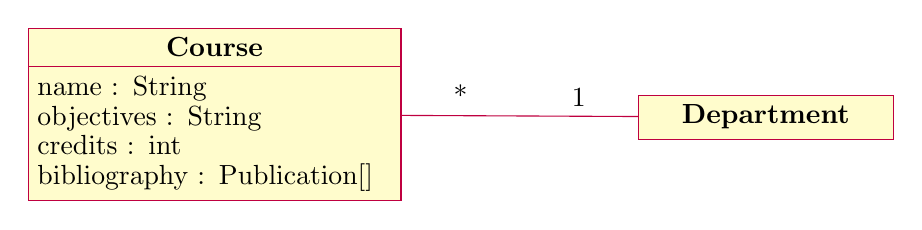
\begin{tikzpicture}

\begin{class}[text width=4.5cm]{Course}{0.5,0}
  \attribute{name : String} \attribute{objectives : String}
  \attribute{credits : int} \attribute{bibliography : Publication[]}
\end{class}

\begin{class}[text width=3cm]{Department}{7.5,-0.85}
\end{class}

\association{Department}{}{1}{Course}{}{*}

\end{tikzpicture}

\caption{Sample Domain Model in UML}
\label{fig:courseDomain}

\end{figure}

In this simplified domain model, a course belongs to a department, has
a name, its objectives, the credits granted upon completion, and the
recommended bibliography. The domain is deemed to be consistent only
if all attributes of course have a defined value. Each department is
responsible for managing its courses. The creation of a new course
should be executed transactionally, because other users of the system
should not be able to see a course in an inconsistent state. There are
several ways to implement this operation on a web application, using already existing
functionality.

\subsubsection{Business Transaction in a single interaction}

A possible implementation of the course creation operation is to have
a single page in which the user provides all the required
information. Once the information is submitted, a new \texttt{Course}
is created and all its attributes are filled according to the
information submitted by the user. The new object is then stored in
the database, making it persistent and available for other users to
view.

In this scenario, the transactional guarantees of the operation are
ensured by the underlying database (which is assumed to provide the
classic transactional semantics \cite{gray1981transaction}), because
the whole operation can be performed within the scope of a single
database transaction. An important consequence of implementing the
operation in a single database transaction is that the programmer can
manipulate all the domain objects involved directly. The order in
which the modifications to the objects are performed is irrelevant, as
long as the domain is consistent when the transaction is
committed. This is the semantics typically expected by a programmer of
such applications: There may be instants in which some domain objects
are in an inconsistent state, but this inconsistent state will never
be seen by the other users of the application. Those users will see
the fully created object only when the operation is committed.

\subsubsection{Business Transaction across multiple interactions}

The model described in the previous scenario may not be suited for
every situation. Imagine that instead of four attributes,
\texttt{Course} had 50 attributes. It would then be unfeasible to ask
the user to fill everything out in a single web page. One possible
solution would be to split the various attributes in multiple pages,
accounting for multiple user interactions. 

At first glance, it would seem quite easy for a programmer to change
the logic programmed in the first scenario to meet the new
requirements: The programmer would simply have to split the code
performed in a single request into smaller parts, each to be executed
in one request. Yet, having separate requests implies having different
database transactions, breaking the atomicity and isolation of the
operation. After handling the first request, the persisted domain
would be in an inconsistent state (a course without all attributes
filled). The implementation of the business logic must then take this
issue into account, because the programmer cannot write the updates
directly on the domain. This scenario represents what was defined as a
Long-Lived Transaction, in which the Business Operation has a larger
lifetime that a single database transaction.

\subsection{Why are they difficult to implement?}
\label{sec:difficult}

In this multiple interaction scenario, the programmer must take
special care when implementing the operation. There are several
possible approaches available:

\subsubsection{Keeping a database transaction open}

Given that atomicity and isolation are broken due to the fact that
each interaction with the user is done within its own database
transaction, we could think that the solution would be to keep the
database transaction open during the whole business
transaction. However, most modern Relational Database Management
Systems (RDBMSs) do not cope well with transactions that are open for
arbitrarily large periods of time, because a long lived database
transaction may limit concurrency, cause timeouts and deadlocks or
starve the database's connection pool. All these factors contribute to
making this approach highly undesirable, making the programmer seek
alternative approaches.

\subsubsection{Parallel Representation of the domain}

In this approach, a series of manually managed objects similar to the
domain objects are created and kept outside the domain. As the
complexity of the domain and the number of objects manipulated by the
operation grows, it becomes harder for the programmer to manage
manually all of the data that must be kept. Ultimately, there is a
copy of the whole domain stored in the user's session, waiting for the
last transaction to update the domain with all the information entered
by the user. This is the opposite of what would be desirable for the
programmer: It should possible to operate directly on the domain.

\subsubsection{Changing the domain model}

Now imagine that the course creation process can span several
days. Keeping the data in the user's session is not feasible, as the
system may restart and discard the written information. This means
that the intermediate data must be manually kept persistently.  A
possible solution for this is to change our domain model, by adding a
new attribute to the objects being modified. The \texttt{status}
attribute would indicate whether the course is in a consistent state
(\texttt{Published}) or not (\texttt{Draft}). Adding this attribute
has a cost: Not only the domain becomes polluted with information that
is not relevant to the object being modeled, but this solution affects
other functional code across the application (e.g., course listings
must filter out courses that are still in the \texttt{Draft} status),
scattering the filtering code throughout the application.

\subsection{Objectives}

Implementing Long Lived Transactions using current transaction support
systems is a rather difficult task that promotes poor software
engineering practices. As such, the work presented in this
dissertation aims at providing a solution that: (a) Survives system
restarts, ensuring that the intermediate data is always available, (b)
Provides the same correctness guarantees as regular transactions, (c)
Allows multiple users to collaborate concurrently on the execution of
a Long Lived Transaction, (d) Does not impose an overhead on the
execution of regular transactions and (e) Shows performance results
comparable to those of regular transactions.


%% Related Work

\section{Related Work}
\label{chap:related}

In this section I describe the various areas in which an attempt to
solve the problem of Long Lived Transactions has been made, namely
Database Management Systems, Workflow Systems, and Object-Relational
Mapping Systems.

Also, due to its relevance regarding the solution described in section
4, I briefly present Software Transactional Memories (STM), Nested
Transactions, Persistent STMs, and how they cope with short lived
transactions.

\subsection{Transactions in Database Management Systems}
\label{sec:rdbms}

Transactions are an age-old notion in the database world. They
comprise a {\it Unit of Work} performed within a Database Management
System, and ensure that concurrent access to shared mutable data is
done in a consistent way.

A database transaction typically provides the four ACID properties:
Atomicity, Consistency, Isolation and durability.

\subsubsection{Concurrency Control}

Concurrency Control is the mechanism that ensures that ``Concurrent
execution should not cause application programs to malfunction''
\cite{reuter1993transaction}. This property was coined in 1993 as the
first law of Concurrency Control, by Jim Gray. In fact, concurrency
control mechanisms are what ensure that the ACID properties of
transactions are kept, in an environment with concurrent access to
shared mutable data. Research on the topic dates back to the 1970s
\cite{rosenkrantz1978system} and 1980s \cite{gray1981transaction}, and
is still a hot topic nowadays.

There are two main categories of Concurrency Control: Optimistic and
Pessimistic. {\bf Optimistic} consists on delaying integrity checking
until the end of the transaction, without blocking any of its reads
and writes. As the integrity of the operation is only checked at the
end of the transaction, conflicts are not detected until all the work
is done and the transaction has to be restarted. It is typically
implemented by Multiversion Concurrency Control and Timestamp Ordering
mechanisms \cite{Bernstein1981}. {\bf Pessimistic} Implies that every
data access in the transaction acquires a lock before
proceeding. During the acquisition process, if an integrity violation
is detected, the transaction is aborted, rolling back every write and
releasing every lock held. Once the transaction is finished, it is
marked as committed, and all the locks are released. Historically,
pessimistic concurrency control has been the dominant category, and
even nowadays, most Relational Databases implement it. Due to this
fact, most of the work regarding Long-Lived Transaction support in
DBMSs is related with locking approaches. In fact, one of the main
reasons why databases do not cope well with long transactions, is that
the transaction holds a lock for each accessed record.

\subsubsection{Relaxation of Transactional Properties}

Given that holding the locks for the duration of the transaction was
not viable, the first proposed solution for this problem was to accept
a lower degree of consistency, by allowing transactions to release
their locks before commit. In \cite{gray1981transaction}, the author
proposed a model in which only {\it active} transactions (the ones
currently updating the database) hold locks. {\it Sleeping}
transactions (not currently updating the database - also known as {\it
  User Think-Time}) do not hold any locks. This means that the
isolation property is broken, due to the fact that other transactions
will be able to see an uncommitted value.

In \cite{salem1989altruistic}, the authors propose an extension to
Two-Phase locking, called {\it altruistic locking}. This extension
provides the concurrency control manager with a set of rules that
allow it to release locks early in the transaction. The altruistic
protocol takes advantage of the knowledge that a transaction no longer
needs access to a data object that it has locked. Transactions can
then issue {\it release} operations, indicating that a certain piece
of data will no longer be accessed. Other transactions will be allowed
to access this data concurrently, while agreeing to abide by certain
restrictions that were put in place to ensure that all transactions
see a consistent database state.

\subsubsection{Transaction Logs}

Typical DBMSs keep a Transaction Log, keeping a record of every
operation, so that crash recovery can be performed. The problem is
that the size of that log is finite and, over time, it fills up, thus
forcing Long-Lived Transactions to abort, as some of their log records
will be overwritten by more recent transactions. In
\cite{hagmann1991implementing}, the authors propose ``Log Record
Forwarding'', as a means to relocate log entries belonging to
Long-Lived Transactions, so that they will not be aborted for that
reason. In this proposal, active records in the log area are copied
(forwarded) to the end of the log, thus surviving another
log-reclaiming cycle.

\subsubsection{Sagas}
\label{sec:sagas}

Garcia-Molina and K. Salem proposed the notion of sagas
\cite{garcia1987sagas}. The basic idea of the saga model is to allow a
transaction to release resources prior to committing. A Long-Lived
Transaction is a saga if it can be seen as a sequence of
sub-transactions that can be interleaved in any way with other
transactions. Each sub-transaction in the saga guarantees that the
ACID properties on the database are preserved. Partial executions of
the saga are undesirable, so the DBMS is responsible for guaranteeing
that either all transactions in a saga are successfully completed, or
compensation actions are run to amend the partial execution. Thus,
each sub-transaction is associated with a compensating transaction,
which undoes the changes performed by the original transaction. Note
that this action does not necessarily return the database to its
original state, but instead acts upon the {\it business state} of the
application.

\subsubsection{Offline Concurrency Patterns}

In \cite{fowler2003patterns}, Martin Fowler introduced a series of
{\it Offline Concurrency Patterns} as the building blocks for
Long-Lived Transactions using simple DBMS-provided regular
transactions. In the book, the author presented the concept of {\it
  Optimistic} and {\it Pessimistic} Offline Locks, as
application-level workarounds to support Long Lived Transactions.

The {\bf Optimistic Offline Lock} solves the problem by validating
that the changes about to be committed by one session (or business
transaction) do not conflict with the changes of another session. This
is achieved by, once the session is being committed, validating that
the changes about to be committed are consistent, making sure that the
value previously read by the current session was not changed by
another session (i.e. obtaining an Optimistic Offline Lock). If the
version cannot be validated, a conflict is detected and the LLT is aborted.

The {\bf Pessimistic Offline Lock} prevents conflicts by avoiding them
altogether. It forces a business transaction to acquire a logical lock
(in a specific lock table) in each record before using it, so once you
begin the business transaction, you are mostly sure that it will
complete without concurrency control issues.

Although with the use of these patterns the development of Long-Lived
Transactions is facilitated, they require the programmer to pollute
the domain with the addition of code that should be at an
infrastructural level.

\subsection{Workflow Management Systems}

A Workflow Process is described as a sequence of connected steps (or
activities), with special emphasis on the flow paradigm, where each
step of the process follows the precedent, and ends just before the
next step can begin. A Workflow Process typically may have a long
duration and involve many users. It should be clear that a Workflow
Process presents many similarities with a Long Lived Transaction, and
as such, may be a suitable solution to implement them. However,
Workflow Processes are not concerned with the ACID properties in the
same way as DBMSs. Instead, they let the intermediate state of the
ongoing processes be visible to the outside world, and rely on
compensatory actions to be executed in case a process fails and has to
be rolled back. This isolation breach is not acceptable for the
problem at hand, and as such, Workflow Management Systems are not
suitable to implement Long Lived Transactions.

\subsection{Object-Relational Mapping}
\label{sec:orm}

Due to the increase in popularity of object-oriented programming, a
large number of Object-Relational Mapping (ORM) tools have arisen over
the past few years \cite{orm}. These tools provide an object-oriented
view of the database, making it completely transparent to the
programmer. To provide transactional support for domain objects, ORMs
typically delegate transaction management to the underlying Database
(which is assumed to provide full ACID support). Thus, Long-Lived
Transaction support in ORM tools is largely dependent on the
underlying DBMS.

The specification of the Java Persistence
API\footnote{\texttt{http://jcp.org/en/jsr/detail?id=317}} (JPA)
assumes the use of optimistic concurrency control (or optimistic
locking). In this context, optimistic locking is used to prevent the
database from holding on to critical resources, potentially causing
high degrees of contention.  This is achieved by operating directly on
the domain objects (in memory), delaying the propagation of the
changes to the database as much as possible. As part of the JPA, there
is the concept of Version field. This field allows {\it disconnected
  operation}, meaning that the reads/writes from the database are
deferred until a checkpoint or the end of transaction.

Hibernate supports the concept of {\it Long Conversations} by allowing
a session to remain open as long as the user interaction lasts,
potentially executing multiple database transactions. However, the
programmer is responsible for ensuring the atomicity and isolation of
the business transaction, by following a very strict pattern: All
transactions but the last must only read data. Hibernate assists the
programmer in verifying that the data read across the multiple
transactions is consistent, using an object versioning
mechanism. This, however, requires that all data be read in the first
transaction. This support is far from our requirements as it imposes a
pattern that may not be suited for many applications.  All the state
of the transaction is kept in memory, which may cause the application
to run out of memory in very large transactions. Despite the
versioning support, the business transaction may still suffer from
inconsistent reads, as it spans multiple isolated database
transactions.


\subsection{Software Transactional Memories}
\label{sec:stm}

The original idea behind Transactional Memories (TM)
\cite{herlihy1993transactional} is to provide efficient lock-free data
structures for highly concurrent systems using hardware. Its main goal
was to free programmers from using locks and monitors to manage
concurrent accesses to shared data. Over the years, the original
concept of Hardware Transactional Memories has evolved, giving birth
to Software Transactional Memories \cite{shavit1997software}. STMs
bring into the realm of programming languages, the age-old notion of
transactions, well-known in the area of DBMSs. However, unlike those,
STMs are not concerned with the Durability property of the ACID model,
and thus, many STM implementations have little in common with their
database counterparts. There have been several recent proposals for
STM implementations, such as those described in
\cite{cachopo2006versioned, herlihy2003software,
  dice2006transactional}.

STMs use transactions to isolate memory operations in atomic Units of
Work. A transaction typically contains a Read Set and a Write Set,
which are used to register its read and write operations,
respectively. The STM provides a series of mutable memory locations
that can be read from or written to. It is the responsibility of the
STM to guarantee that concurrent accesses to such memory locations are
correct according to the specified correctness criteria. In
particular, in \cite{guerraoui2008correctness}, an {\it Opacity}
correctness criteria is defined for STMs.

The best practices in software development encourage programmers to
modularize their applications and have them abide by well-defined
interfaces. Lock-based approaches do not cope well with this
principle, because the programmer must be aware of module's internal
locking conventions. In the transaction paradigm, it would then be
common for application code to make a call to a library that uses
transactions to protect its shared internal state. In this scenario,
the transaction created by the library would be {\it nested} in the
outer (application-owned) transaction. Nested Transactions are an
extension to the basic transaction structure, supporting multiple
levels of transactions: Transactions that may contain other
sub-transactions, forming a transaction tree. Nested Transactions have
long been used in the database world, and many of its concepts have
been adapted to transactional memories. Consider the kind of
monolithic transactions commonly found in enterprise applications. In
such transactions, the volume of work that must be done if the
transaction needs to be rolled-back is increased. Using nested
transactions, smaller portions of the work can be done in isolation,
each within a nested transaction. If one of those portions fails, only
that portion needs to be rolled-back, and an attempt can be made to
compensate for that failure. Nested Transactions present many
similarities with Long-Lived Transactions. In both cases there is a
top-level transaction, which can be divided in several smaller steps.

In \cite{fernandes2011strict}, the authors argue that keeping the
transaction management in the database, while once justified by
hardware limitations, is no longer suited for today modern
applications. A new architecture was proposed, using a STM for
transaction support at the application server tier. The database still
plays an important role in this architecture, due to the fact that the
STM must be extended to support persistence (PSTMs).  By shifting the
responsibility for transaction handling to the STM, enterprise
applications can benefit from the many advancements in the STM area,
such as multi-core machine scaling, stronger correctness guarantees
and nonblocking progress conditions such as lock freedom.  Using a
PSTM, enterprise application developers no longer have to trade
correctness for performance.

Another advantage of PSTMs is that, the programmer benefits from a
much simpler and transparent programming model, allowing for much
cleaner and maintainable code, better composability, making the
process of translating business requirements to code much simpler and
bug-free. This work aims at extending the PSTM model with Long Lived
Transaction support.

%% FF

\section{Fenix Framework}
\label{chap:ff}

This section briefly describes the Fenix Framework, which is the
Framework used to implement the solution proposed throughout this
document. The information presented in this section is critical to
understanding the proposed solution, as well as its challenges.

\subsection{Domain Modelling Language}
\label{sec:dml}

The Domain Modelling Language (DML) is a Domain-Specific Language
designed to represent object-oriented rich domain models, separating
the domain's structure from its behaviour. The DML is designed with
modularity as a core concern, allowing for incremental and modular
domain definition.

In a DML file, programmers write their domain definition in a
Java-like language. A class definition consists of the class name, the
entity slots, and the super class. Relations in DML are named,
first-class citizens that represent relationships between two
classes. Relations are always bi-directional, meaning that updating
one side of the relation will automatically update the other
side. Relations can be concealed in one of the sides (meaning that it
will not be possible to access it), however their state is still kept.
It is possible to define {\it one-to-one}, {\it one-to-many} and {\it
  many-to-many relationships}. To-many relations in the Fenix
Framework have Set semantics, meaning that an object can only be
present in a relation once.

From the domain definition, the Fenix Framework generates Java getters
and setters for the properties and relations. For each class described
in the DML, two Java classes are created: the domain class, in which
programmers can include business logic, and a \texttt{Base} class
(which the domain class extends) containing generated methods to
access the persistent entities of the object.

In the DML there is a distinction between entities and value
objects. Value Objects are immutable and not persistent by
themselves. They are used as the values for slots of DML classes, and
must be of well-known types, known as Value Types. A value type
contains information regarding the Java Type an alias and information
regarding how the object will be externalised/internalized.

\subsection{Architecture}
\label{sec:ff-arch}

The Fenix Framework's architecture provides a clear separation between
the Framework's public API and the transactional/persistence
backends. The programmer writes his application against a public API
and is able to run it on multiple backends. This way, not only are
applications portable across several technologies, but also testing
support is greatly enhanced, as it is able to simply plug a transient
persistence support.

The \texttt{DML Compiler} module contains the parser responsible for reading
DML files and creating an in-memory description of the Domain Model,
as well as all the necessary classes to represent it. It also contains
the base \texttt{DomainObject} interface, which all objects of the Domain
Model implement. Also present in this module are the base Code
Generators used to create the Base classes for all domain
objects.

The core of the Framework is in the \texttt{Core API} module. Transaction
management APIs, configuration, entry points, backend interfaces, are
all defined in this module.

The \texttt{DML Compiler} and \texttt{Core API} modules are the Fenix
Framework's public API, providing everything necessary to the
development of backend-independent application modules.

Backends are a crucial part of the Fenix Framework. They provide
concrete implementations of the transactional and persistence
support. Application modules should not depend directly on the
backends, as their API is private and as such subject to change even
among minor versions, and having a dependency on a specific backend
means that portability must be sacrificed.

\subsection{JVSTM}
\label{sec:jvstm}

The Java Versioned Software Transactional Memory (JVSTM)
\cite{cachopo2006versioned} is a pure-Java implementation of a
Software Transactional Memory (see Section~\ref{sec:stm}).  It uses
the concept of Versioned Boxes (VBoxes) to make a memory location
transactional, keeping the history of values for that position, one
for each version of the box. Each transaction has a version number
that is used during the transaction to ensure that all reads get the
correct value at the time of the transaction's star. This allows for
conflict-free read-only transactions, as concurrent transactions
writing to the read boxes will write a new version instead of
overwriting its previous value.

The JVSTM is integrated with the Fenix Framework, as one of the
multiple available backends. This document focuses on the backend
named \texttt{jvstm-common}, on top of which the solution will be
developed. This backend uses the JVSTM for the transactional support,
while abstracting the persistence details. Despite being meant to be
extended, \texttt{jvstm-common} provides an in-memory implementation
of the persistence API.

A plain JVSTM VBox is simply a wrapper to a Linked-List of pairs
[Version, Value], containing the history of values for that box. In
the Fenix Framework, VBoxes are specialised to hold the value of an
object's slot (persistent slot declared in the DML). A Fenix Framework
VBox contains a back-pointer to its owner, as well as the name of the
slot it represents. This allows for the persistence support to know
where to store the value of the Box.  Those specialised VBoxes can
have their previous values Garbage-Collected and reloaded from
persistent support on-demand. In terms of VBoxes, {\it to-one}
relations are treated just like any other slot, and as such, the
reference to the related object is simply kept within a regular
VBox. To-many relations however, are handled in a very different
manner. The preferred approach is to use a B+Tree
\cite{elmasri2009fundamentals} to store the objects on the to-many
side of the relation. For each to-many relation, a VBox is generated,
referencing the domain object representing the B+Tree.

%% Solution

\section{Solution}
\label{chap:solution}

With a proper understanding of the Fenix Framework, this section
describes the solution proposed to simplify the development of Long
Lived Transactions.

\subsection{Architecture}
\label{sec:arch}

The main goal of this work is to relieve programmers of the burden of
dealing with Long Lived Transactions, making the effort needed to
program an LLT similar to the effort of programming a regular
transaction. So, what does the single interaction scenario has that
makes it so easy to program? It has a single transactional context
that spans the whole operation (provided by the STM transaction). In
the multiple interaction scenario the system transaction was shorter
than the business transaction, so in each step the context was lost.

Looking at the information that is kept during the lifespan of a
regular transaction, we can identify three major pieces: (a) The
version of the LLT (corresponding to the version of the first step),
(b) A list of all the items written throughout the transaction (and
the respective written values) and (c) A list of all elements read
throughout the transaction. This piece of information is critical to
ensure the correctness of the operation.

These pieces are crucial to ensure the correct operation of an
STM-based transactional system. STM libraries provide them for regular
(short-lived) transactions. The solution presented below aims to
provide them for Long Lived Transactions, using the short-lived
transactions as its building blocks. Short lived transactions keep all
the necessary information in transient transaction-local storage
(typically in memory), until the time they commit, merging the write
set with the global state of the application. With Long Lived
Transactions, merging this write set in each step is not possible.

There needs to be a way to persistently store the Write Set of each
step, outside the global state of the application so that the changes
are not visible to the outside world. Only upon committing the Long
Lived Transaction these changes would be merged to the global state,
meaning that the writes performed by each step are effectively delayed
until the end of the transaction. Note that for correctness purposes,
the Read Set of the transaction must also be collected, so that at
commit time both Read Set and Write Set can be replicated, taking
advantage of the already existing JVSTM support.

As the main feature of the Fenix Framework is providing mechanisms to
manipulate transactionally and to persist Domain Objects, perhaps it
would be a good approach to use regular Domain Objects to store the
required information.

\subsubsection{Data Structures}

\begin{figure}
\centering
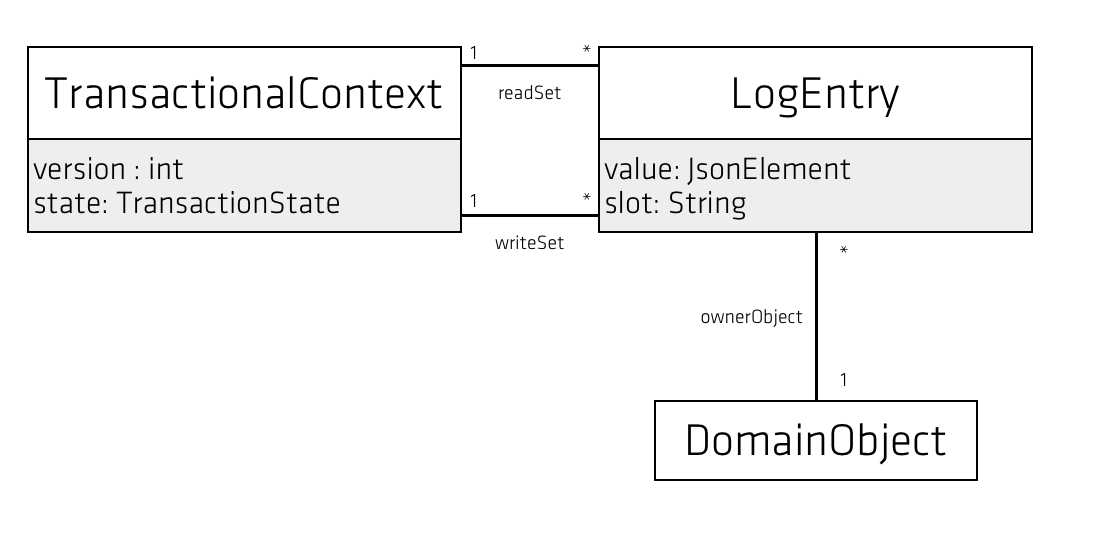
\includegraphics[width=0.5\linewidth]{tx-context}
\caption{Transactional Context's Domain Model}
\label{fig:transactionalContext}
\end{figure}

Consider the domain model presented in
Figure~\ref{fig:transactionalContext} that represents the reification
of the necessary data necessary for a transaction. A
\texttt{TransactionalContext} is the centerpiece of the domain, it
represents a Long Lived Transaction, holding together the entire state
of the transaction. By keeping the state of the LLT in regular domain
objects, we are ensuring that it is stored persistently as well as
transactionally safe. Updates to the context are performed using a
regular transaction, allowing for multiple users to concurrently run
LLT steps.

A \texttt{TransactionalContext} has two associated sets of
\texttt{LogEntries}, one for the Read Set and one for the Write Set. A
\texttt{LogEntry} represents one read or written slot throughout the
transaction, by keeping a reference to the object, slot name, as well
as the value that was written (note that the value is only kept if the
LogEntry belongs to the Write Set).

\subsubsection{Transaction Isolation}

Whereas the data structures are agnostic to the specific backend, the
backend must be able to recognise when a transaction is executing
within the context of a Long Lived Transaction, so that reads and
writes are isolated from the global state of the application
(otherwise the whole world could see the intermediate values).

In the Fenix Framework, transactions are bound to a specific thread,
allowing for multi-threaded applications to execute multiple
concurrent transactions, each one in its own thread. As such, to run a
transaction in the context of a Long Lived Transaction, one must first
bind the context to the current thread. This way, when beginning a new
Transaction, the backend will check for the presence of a
\texttt{TransactionalContext}, to determine whether to start a regular
transaction or a LLT step. Listing~\ref{list:longTxBind} shows the
programmer API for binding a \texttt{TransactionalContext} to a given
thread. This way, the programmer is free to run any piece of
transactional code as a step of a Long Lived Transaction.

\begin{lstlisting}[caption={Example of TransactionalContext usage},
  label={list:longTxBind}]
public void runStep(TransactionalContext context) {
  LongTransaction.setContextForThread(context);
  try {
    transactionalOperation(); // @Atomic method
  } finally {
    LongTransaction.removeContextFromThread();
  }
}
\end{lstlisting}

When reading the value of a slot within a
\texttt{TransactionalContext}, it is the responsibility of the backend
to check whether the slot is in the Write Set of LLT, and if it is
not, read the value of the slot in the correct version (the version
recorded in the context). Slot reads are recorded as a
\texttt{LogEntry} in the Read Set. When writing the value of a slot,
the written value is stored as a \texttt{LogEntry} in the Write Set,
so that it can later be retrieved by read operations and used to
update the state of other domain objects when committing the
transaction. Reads and Writes will be processed, and a set of
\texttt{LogEntries} created.  As such, in the end of a step, only
slots belonging to the \texttt{TransactionalContext} and its
\texttt{LogEntries} are written to persistent support.

\subsubsection{Committing the Long Lived Transaction}

Just like in a regular transaction, a Long Lived Transaction must be
atomic and consistent, meaning that its effects must appear to have
occurred at a single well-defined point in time. To accomplish this,
all elements of the Read Set must be validated to be in the same
version, thus ensuring that all writes were performed based on fresh
data. If the validation step is successful, all the written data must
be merged into the global state of the application, by iterating over
all \texttt{LogEntries} in the Write Set, and writing the recorded
value to the correct slot. To ensure the correctness of the commit
operation, both validation and merge are performed within a regular
transaction, in a backend-specific manner. Any conflicts on this
operation, such as multiple concurrent commit operations, or writes to
validated slots will cause the commit transaction itself to abort and
restart.

Programmers can also manually rollback the Long Lived Transaction. In
this situation, all the information stored in the corresponding
\texttt{TransactionalContext} is deleted. As the Reads and Writes
performed by the transaction are stored exclusively in the context, no
further action is required.

\subsection{Implementation}
\label{sec:impl}

The {\bf long-tx-api} module is the first part of the implementation. It contains
the domain definition described in
Figure~\ref{fig:transactionalContext}. The domain is public API, so
that Long Lived Transactions can be associated with any
programmer-defined object (e.g., to a user, to a group, a process
etc). This design decision allows for a simple solution, as
cross-cutting concerns such as security and sharing are abstract, and
also gives the programmer more flexibility.

The \texttt{jvstm-common} also needed several modifications to support
LLTs. The following sections describe those modifications.

\subsubsection{Context Detection}

When beginning a transaction in \texttt{jvstm-common}, the backend
checks for the presence of a \texttt{Transactional Context} bound to
the current thread, and if one is present, the following happens: (1)
A regular transaction is started. This transaction will be used to
access the context and previous versions of VBoxes (for when a read is
made and the context cannot provide a value). (2) A nested
\texttt{LLTStepTransaction} is started. This will be the active
transaction, and route reads and writes to the corresponding
\texttt{TransactionalContext}. (3) In case this is the first step of
the LLT, it is necessary to define its version. To ensure that every
other step of the LLT has the same view of the world as this one, mark
the LLT's version as the version of the current transaction.

The main reason to use a Nested transaction is to allow portability
across concrete persistence implementations, as the
\texttt{LLTStepTransaction} will be agnostic to the specific
underlying transaction (provided it fulfils the required API). A
\texttt{LLTStepTransaction} holds a reference to the
\texttt{TransactionalContext} backing it, so that it can perform
searches in the context's Write Set.

\subsubsection{Intercepting Reads and Writes}

As in the JVSTM backend each domain object slot is backed by a VBox,
intercepting reads and writes to slots can be easily done. The
implementation of the get/set methods in a VBox simply delegates the
read/write to the current transaction, which conveniently, is a
\texttt{LLTStepTransaction}.

Just like in regular transactions, writing a VBox will simply keep the
written value in the transaction's Write Set. This Write Set will be
processed when committing the step.

When reading a VBox within a \texttt{LLTStepTransaction} the following
steps are executed: (1) If the VBox was previously written in this
step, return the written value. (2) In case the VBox being read is
owned by either a \texttt{TransactionalContext} or a
\texttt{LogEntry}, the read is delegated to the parent transaction in
the current version (This is required for correct behaviour). (3) If
the VBox was written in a previous step of the Long Lived Transaction,
return the previously written value, obtained from a \texttt{LogEntry}
in the Write Set of the LLT.  Else, delegate the read to the
underlying transaction, in the same version as the context, and add
the VBox to the current transaction's Read Set.

When the transaction finishes, the \texttt{LLTStepTransaction} has in
its Read and Write Sets the actual VBoxes that were read/written
during the transaction. Recall that in each step the Read Set and
Write Set of the step must contain only the changes to the context
that reflect what has been read and written. As such, when committing
the step, the Read Set and Write Set are processed in the following
manner: (1) The parent transaction is set as the current
transaction. (2) For each item in the original Write Set, the written
value is added to the \texttt{TransactionalContext}. As this operation
runs within the parent (backend-specific) transaction, the newly
created and updated \texttt{LogEntries} are added to the Read and
Write sets of the parent transaction. (3) The same is done to the Read Set.

Once the nested transaction is committed, the parent
(backend-specific) transaction will ensure that the updated
\texttt{TransactionalContext} is stored in persistent support. Note
that the only objects written in the parent transaction will be the
ones representing the context and its \texttt{LogEntries}.

\begin{figure}
\centering
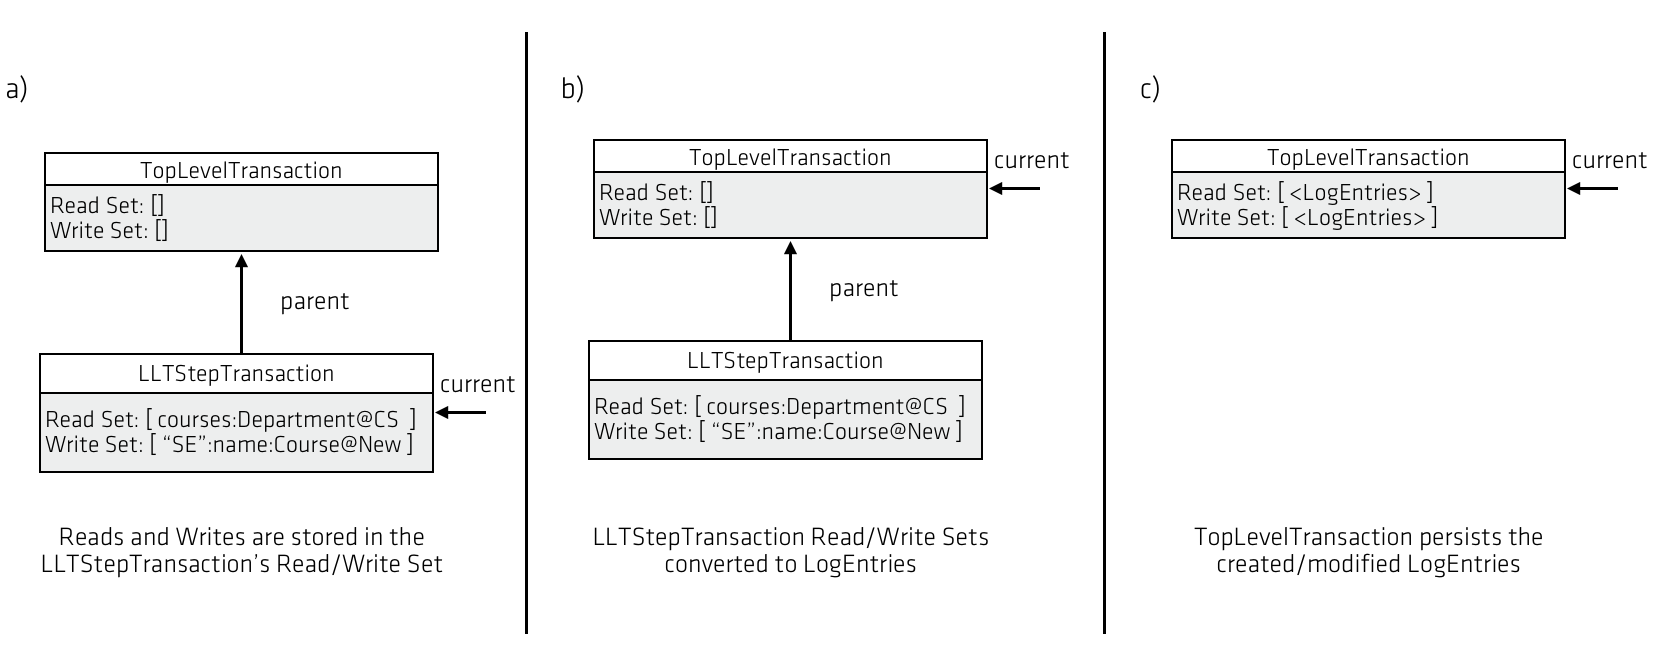
\includegraphics[width=.9\linewidth]{llt-step-lifecycle}
\caption{LLTTransactionStep lifecycle}
\label{fig:llt-lifecycle}
\end{figure}

Figure~\ref{fig:llt-lifecycle} recaps the lifecycle of a
\texttt{LLTStepTransaction}.

\subsubsection{Finishing the Long Lived Transaction}
\label{sec:jvstm-commit}

Once all steps of the Long Lived Transaction are finished, the LLT
must be committed, ensuring that the changes performed in it are
visible to the outside world.

The commit process of a Long Lived Transaction occurs within a regular
transaction. In this process, the data collected throughout the
multiple steps is validated and replayed. Once this transaction
commits, all written data will be merged with the global state of the
application.

The first step in committing the LLT is verifying whether all the read
data is still valid. As every slot is mapped in a JVSTM VBox, all the
boxes corresponding to the read slots must be verified. The process
iterates over all read slots, locating the VBox that represents the
slot. It then reads the VBox, so that it is added to the Read Set of
the current transaction. Then, the latest version of the VBox is
compared to context's version, thus ensuring that the read value was
the latest. If the box's current version if posterior to the read
version, the Long Lived Transaction is aborted.

There is a critical subtlety in this verification
process. Modifications to the VBox's underlying data structures are
performed only at commit time, inside a commit lock. As the
verification process is not run within the commit lock, it is possible
for another transaction to concurrently update a VBox after the
validation. Preventing incorrect behaviour is quite simple: Just read
the box. By doing this, the box will be validated when the transaction
commits, ensuring that the verification was correct (i.e. the version
read during the verification is still valid).

Once the Read Set of the Long Lived Transaction is validated, the
Write Set must be merged into the global state of the
application. This process iterates over the written slots, and for
each slot: (1) Locates the VBox representing it, (2) Converts the JSON
value to the concrete value, and (c) Writes the value to the VBox.

After the merge process is finished, the committing transaction has a
full mirror of the LLT's Read and Write Sets, and once it commits,
every change in the Write Set is available to the outside world.

\subsection{Validation}
\label{sec:validation}

This section proposed a solution that allows programmers to take
advantage of Long Lived Transactions with little effort and no code
modifications. I will now show how the solution fares in each of these
aspects.

\subsubsection{Correctness}

One of the greatest challenges when implementing Long Lived
Transactions is ensuring that the solution provides the same
correctness guarantees as regular transactions. Transactions in the
JVSTM satisfy the Opacity correctness properties
\cite{guerraoui2008correctness}. The proposed solution provides all
the ACID properties for Long Lived Transactions, as well as the
Opacity correctness property.

Throughout the execution of the Long Lived Transaction, written data
is collected and stored inside the \texttt{Transactional Context}. Once
the transaction is finished, written data is {\bf atomically} written
to the global context, using a regular transaction which simply reads
data from one domain object to be written in another.  Long Lived
Transactions are {\bf consistent}. Similarly to regular transactions,
a LLT only commits if all the data read during the transaction is
still valid at commit time, performing a validation similar to that of
regular transactions.

{\bf Isolation} is perhaps the hardest property to demonstrate. When
performing a read operation within a Long Lived Transaction, the
system ensures that the returned value will be the one at the moment
the first step of the LLT executed (i.e. the value consistent with the
transaction's version), just like it happens with regular
transactions.  As for writes, similarly to what happens with regular
transactions, written values are kept in transaction-local storage
(i.e. in \texttt{LogEntries}) and as such, can only be accessed by the
transaction itself.

\subsubsection{Ease of Use}

The primary goal of this work is to ease the development of Long Lived
Transactions, and as such, it is rather important to provide a simple
and concise API. The proposed solution fares well in that regard, as
it allows existing code to be adapted to use Long Lived Transactions
with no modifications. It is possible to program the business logic of
your whole application using regular transactions, and with a simple
wrapper add Long Lived Transaction support.

Consider a Web Application wishing to share with its users the
benefits of Long Lived Transactions, by allowing each individual user
to keep a series of Long Operations. Making every action performed by
the user as a step of the Long Lived Transaction would be as simple as
keeping the context in session-local storage, and binding it before
every transaction start.


%% Optimization

\section{Optimization}

The proposed solution fullfils all the functional requirements,
however, performs poorly even in trivial test cases (See
Figure~\ref{fig:longv1}). To perform accurate measurements, I
developed a sample banking application. This application is a
simplified model in which there are Customers and Accounts, among
which money can be transfered. In this fictitious scenario, a Business
Transaction will consist of several banking transactions, spread
throughout a series of Business Operations (each operation executes in
its own transaction). To test the performance of the solution, the
transactions are run within the context of one large Long Lived
Transaction.

Figure~\ref{fig:comparisonFinal} shows the running time for a varying
number of operations of the application presented above.  When looking
at the performance of the Long Lived version (where every operation is
a step of one large Long Lived Transaction), performance quickly
degrades as the number of operations grows. The main reason for this
performance hit is that every box read will cause many other boxes to
be read (instead of just reading the box directly, all LogEntries
representing the write set must be traversed). Recall that each slot
of an object is kept in a separate box, and as such reading a single
Log Entry will cause several boxes to be read. However,
\texttt{LogEntries} belonging to the Read Set have no need for the
value slot, as they only exist to signal that a specific slot of a
specific object was read. The Read Set need only keep pairs
[DomainObject, SlotName], and using \texttt{LogEntries} just for that
is rather expensive. As such, the Read Set has been replaced by an
immutable ValueType, containing a set of DomainSlotKey's (an
immutable, lightweight object representing the pair [DomainObject,
Slot]), stored directly into the \texttt{TransactionalContext}.

The Fenix Framework uses B+Trees to implement {\it to-many}
relations. These collections are transparently handled by the
Framework, and are implemented using regular Domain Objects. As
keeping track of changes in relations is a requirement for our
implementation, it is critical that changes to B+Trees are correctly
tracked. This meant that in the original implementation, the relations
between the \texttt{TransactionalContext} and the \texttt{LogEntries}
representing its Read and Write sets could not be done using a regular
{\it to-many} relation. As such, in the initial implementation the
Read and Write Sets were kept in a Linked-List of \texttt{LogEntries},
with a head pointer in the \texttt{TransactionalContext}.  This
approach proved to be quite inefficient, as lookups in the Write Set
were {\it O(n)} in the number of written objects, making it
impractical, as every \texttt{getBoxValue} operation required
potentially traversing the whole list. To solve this issue, a
specialised \texttt{WriteSetBPlusTree} was developed. The major
difference between a \texttt{WriteSetBPlusTree} and a regular B+Tree
is that the former is designed to be kept out of the scope of the
TransactionalContext, making it possible to use it to implement the
one-to-many relation between a TransactionalContext and its
LogEntries. In Figure~\ref{fig:comparisonFinal} we can see that the
running time using BPlusTrees is closer to the regular
version. 

This approach, however, brought another issue. Despite having great
lookup times, the commit of a Long Transactions's step was greatly
affected. Whereas inserting elements in a Linked List is {\it O(1)},
the insertion in the BPlusTree was rather slow. This is because the
implementation of the BPlusTree does not support batch insertion, and
each insert requires a part of the tree's internal structures to be
duplicated. To solve this issue, the B+Tree was replaced with an
immutable ValueType, containing the mapping between all written slots
and their respective values. With this change, \texttt{LogEntries}
were completely taken out of the picture, as the only extra piece of
information they provided was the JSON contents of the slot, which
could be embedded directly into the WriteSet object. The issue with
this approach is that, due to the immutability requirement, every time
a batch of entries was inserted, the whole Map had to be duplicated,
which was rather wasteful both in terms of time and allocated
memory. So, instead of duplicating the whole Map, the WriteSet is
actually a Linked-List of Maps, containing one node per transaction
step. This means that the performance of lookups is now {\it
  O(s*log(n))}, {\it n} being the average size of each step, and {\it
  s} the number of steps (in which something is written) of the
transaction. This solution provides quite competitive results, with a
slow down of under 40\%.

\begin{figure}
\centering
\begin{minipage}{.5\textwidth}
  \centering
  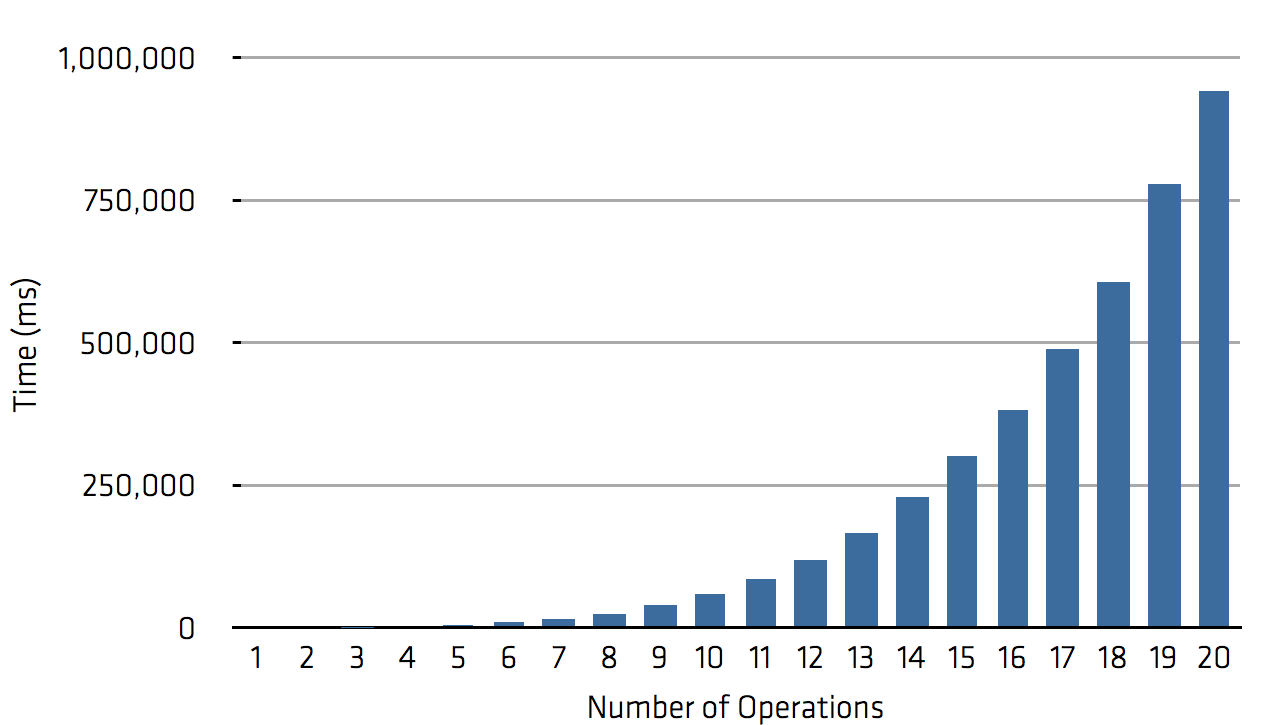
\includegraphics[width=1\linewidth]{time-long-v1}
  \caption{Running time with Long Lived Transaction steps}
  \label{fig:longv1}
\end{minipage}%
\begin{minipage}{.5\textwidth}
  \centering
  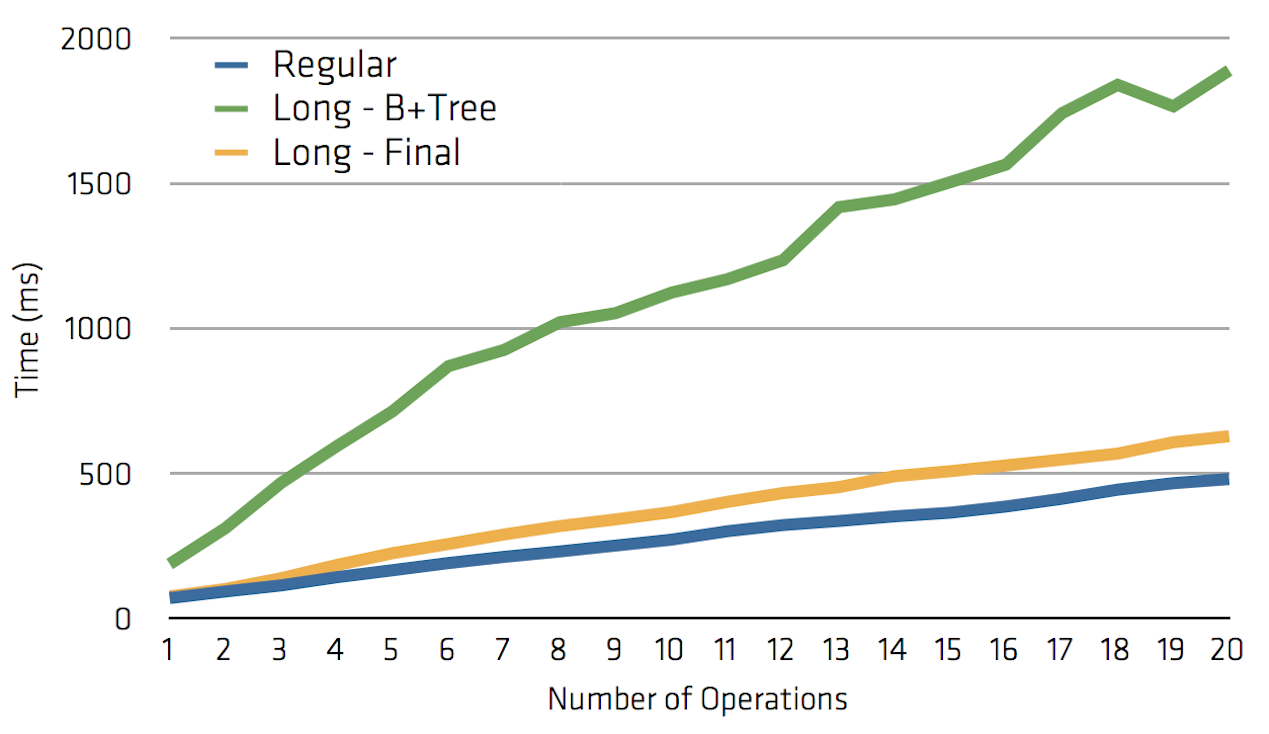
\includegraphics[width=1\linewidth]{3-way-times}
  \caption{Running time comparison for the Final Implementation}
  \label{fig:comparisonFinal}
\end{minipage}
\end{figure}

%% Conclusion

\section{Conclusion}

Many enterprise applications have requirements involving operations
that may span arbitrarily long periods of time. Yet, most modern data
persistence frameworks are lackluster in regard to Long Lived
Transactions. This forces programmers to devise clever ways to
implement their requirements, promoting bad engineering practices and
adding unnecessary complexity to the system.

The Fenix Framework, as a Framework to support enterprise applications
that require a persistent and transactional rich domain model, merely
provided support for regular (short-lived) transactions, and as such,
suffered from the same perils of many other frameworks.

This document has described an extension to the Fenix Framework that
allows drop-in support for Long Lived Transactions, without the need
to modify existing business code. The presented extension shows many
characteristics desirable of such a solution. These include support
for system restarts by storing intermediate data persistently, support
for concurrent users collaborating on a single Long Lived Transaction,
the same correctness guarantees as regular transactions as well as
comparable performance on the execution of the transaction's
steps. The initial implementation, while fully functional, present
very poor performance results, rendering even the simplest of test
cases unusable. I then presented a performance analysis and described
several optimizations that were applied.

\bibliography{biblio.bib} \bibliographystyle{plain}
\end{document}